%\documentclass[letterpaper,draft]{beamer}
\documentclass[letterpaper,handout, mathserif]{beamer}
%\documentclass[letterpaper]{beamer}

%---multiple pages on one sheet, ADD for handout--
%\usepackage{pgfpages}
%\pgfpagesuselayout{4 on 1}[letterpaper, landscape, border shrink=1mm]
%-------------------------------------------------
\usepackage{amsmath,amsfonts}
%\usepackage{booktabs}
%\usepackage{mdwlist}
\usepackage{amsfonts}
%\usetheme{Copenhagen}
%\usetheme{warsaw}
\setbeamertemplate{navigation symbols}{}
\usepackage[english]{babel}
\def\ul{\underline}
% or whatever

\usepackage[latin1]{inputenc}
\subject{Talks}

\def\Sum{\sum\nolimits}
\def\Prod{\prod\nolimits}
\def\p{\mathrm P}
\def\E{\mathbb E}
\def\V{\mathrm Var}
\def\X{\mathcal{X}}
\def\typo#1{\alert{#1}}
%-------------Answers------------
\def\Hide#1#2{\ul{~~~\onslide<#1>{\alert{#2}}~~~}}
\def\hide#1#2{\ul{~~\onslide<#1>{\alert{#2}}~~}}
%------Centered Page Number------
\defbeamertemplate{footline}{centered page number}
{%
  \hspace*{\fill}%
  %\usebeamercolor[fg]{page number in head/foot}%
  %\usebeamerfont{page number in head/foot}%
  \small Lecture \chapnum\ - \insertframenumber%
  \hspace*{\fill}\vskip2pt%
}

%\usepackage{tikz}
%\usebackgroundtemplate{%
%\tikz\node[opacity=0.3] {\includegraphics[height=\paperheight,widht=\paperwidth]{ctanlion}};}

%\usebackgroundtemplate{%
%  %\rule{0pt}{\paperheight}%
%  \parbox[c][\paperheight][c]{\paperwidth}{\centering\includegraphics[width=.65\paperwidth]{UClogo.pdf}}
%  %\hspace*{\paperwidth}
%}

\def\chapnum{15}
%--------------------------------
\setbeamertemplate{footline}[centered page number]

\title{STAT253/317 Lecture \chapnum} \date{} \author{Cong Ma}
\begin{document}
% ----------------------------------------------------------------------
\begin{frame}\maketitle\begin{center}7.3. Limit Theorems\end{center}\end{frame}
% ----------------------------------------------------------------------
\begin{frame}{7.3. Limit Theorems}
Let $\{N(t),t\ge 0\}$ be a renewal process with i.i.d interarrival times $X_i$, $i=1,2,\ldots$ and $\E[X_i]=\mu$.\par\medskip

Explicit forms of $N(t)$ and $m(t)=\E[N(t)]$ are usually {\em unavailable}.
However the limiting behavior of $N(t)$ and $m(t)$ is useful and intuitively makes sense.\medskip

As $t\to \infty,$
\begin{itemize}
\item $\displaystyle\frac{N(t)}{t}\to\frac{1}{\mu}\quad$ with probability 1\hfill (\bf Proposition 7.1)
\item $\displaystyle\frac{m(t)}{t}\to\frac{1}{\mu}$\hfill (\mbox{\bf Thm 7.1\; Elementary Renewal Theorem})
\end{itemize}\bigskip

\underline{Remark.}
\begin{itemize}
\item The number $1/\mu$ is called the {\bf rate} of the renewal process
\item Theorem 7.1 is not a simple consequence of Proposition. 7.1, since $X_n\to X$ w/ prob. 1 does not ensure $\E[X_n]\to\E[X].$
\end{itemize}
\end{frame}
% ----------------------------------------------------------------------
\begin{frame}{$X_n\to X$ Does Not Ensure $\E[X_n]\to\E[X]$}
\mbox{}{\bf Example 7.8}
Let $U$ be a random variable which is uniformly distributed on (0,
1); and define the random variables $X_n$, $n \ge 1$, by
$$
X_n =
\begin{cases}
0 &\text{if }U>1/n\\
n &\text{if }U\le 1/n
\end{cases}
$$
Then $\p(X_n=0)=P(U>1/n)=1-1/n\to 1$ as $n\to\infty.$ So with probability 1
$$X_n\to X=0.$$
However,
$$
\E[X_n]=0\p(X_n=0)+n\p(X_n=n)=n\times\frac{1}{n}=1\quad\text{for all }n\ge 1.
$$
and hence $\lim_{n\to\infty}\E[X_n]=1\neq \E[X]=\E[0]=0.$
\end{frame}
% ----------------------------------------------------------------------
\begin{frame}{Proof of Proposition 7.1}

\vspace{-8pt}\begin{flushright}
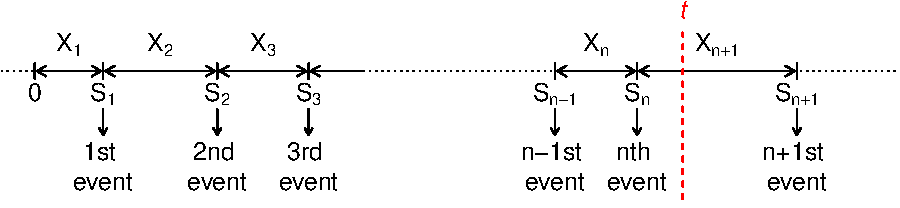
\includegraphics[width=0.4\textwidth, trim=3in 0 0 0 0, clip]{interarrivaltimes.pdf}
\end{flushright}

\vspace{-60pt}
\begin{minipage}{0.7\textwidth}
Since $S_{N(t)}\le t < S_{N(t)+1}$, we know

$$\frac{S_{N(t)}}{N(t)}\le \frac{t}{N(t)} < \frac{S_{N(t)+1}}{N(t)}.$$
\end{minipage}\smallskip

By SLLN,
$\frac{S_{N(t)}}{N(t)} =\frac{\sum_{i=1}^{N(t)}X_i}{N(t)}\to \mu$
as $N(t)\to\infty$,
we obtain $\dfrac{S_{N(t)}}{N(t)} \to \mu$ as $t\to\infty$.
Furthermore, writing

$$\frac{S_{N(t)+1}}{N(t)}=\frac{S_{N(t)+1}}{N(t)+1}\times\frac{N(t)+1}{N(t)}$$
we have that $S_{N(t)+1}/(N(t) +1)\to\mu$ by the same reasoning as before and
$$\frac{N(t)+ 1}{N(t)}\to1\mbox{ as }t\to\infty\quad\text{since}\;P(\lim_{t\to\infty}N(t)=\infty)=1$$
Hence, $S_{N(t)+1}/N(t)\to\mu$.
\end{frame}
% ----------------------------------------------------------------------
\begin{frame}{Stopping Time}
\textbf{Definition.} Let $\{X_n: n\ge 1\}$ be a sequence of independent random variables. An integer-valued random variable $N>0$ is said to be a \structure{\em stopping time} w/ respect to $\{X_n: n\ge 1\}$ if the event $\{N=n\}$ is independent of $\{X_k: k\ge n+1\}.$\medskip

\textbf{Example.} ({\em Independent case.})\\
If $N$ is independent of $\{X_n: n\ge 1\}$, then $N$ is a stopping time.\medskip

\textbf{Example.} ({\em Hitting Time} I.)
For any set $A$, the first time $X_n$ hits set $A$,
$N_A = \min\{n: X_n \in A\}$, is a stopping time because
$$
\{N_A=n\}=\{X_i\not\in A \text{ for }i=1,2,\ldots,n-1,\text{ but }X_n\in A\}
$$
is independent of $\{X_k: k\ge n+1\}$.\par\medskip
\textbf{Example.} ({\em Hitting Time} II.) For $n\ge 1$, let $S_n=\sum_{k=1}^nX_k$.\\
For any set $A$, $N_A = \min\{n: S_n \in A\}$, the first time $S_n$ hits set $A$,
is also a stopping time w/ respect to $\{X_n: n\ge 1\}$ because\smallskip

$\{N_A=n\}=\{\sum_{k=1}^iX_k\not\in A \text{ for }1\le i\le n-1,\text{ but }\sum_{k=1}^nX_k\in A\}$\smallskip

is independent of $\{X_k: k\ge n+1\}$.
\end{frame}
% ----------------------------------------------------------------------
\begin{frame}{Example of Non-Stopping Times}
\begin{itemize}
\item ({\em Last visit time})
The last time that $X_n$ visit a set A \[N_A = \max\{n: X_n\in A\}\] is NOT a stopping time.\\
Clearly we need to know whether $A$ will be visited again in the future to determine such a time.
\item The time $X_n$ reaches its maximum,
\[N = \min\{n: X_n=\max_{k\ge 1} X_k\},\]
is NOT a stopping time since
\[
\{N=n\}=\{X_n>X_k \text{ for }1\le k<n\text{ and }k\ge n+1\}
\]
depends on $\{X_k: k\ge n+1\}$.
\end{itemize}
\end{frame}
% ----------------------------------------------------------------------
\begin{frame}{Renewal Processes and Stopping Times}
Consider a renewal process $N(t)$.
With respect to its interarrival times $X_1$, $X_2,\ldots$,
\begin{itemize}
\item $N(t)$ is NOT a stopping time.
$$N(t) = n \Leftrightarrow X_1 +\cdots+X_n \le t \mbox{ and } X_1 +\cdots+X_{n+1} > t,$$ depends on $X_{n+1}.$
\item But $N(t)+1$ is a stopping time, since
\begin{align*}
&N(t)+1=n \Leftrightarrow N(t)=n-1\\[-3pt]
&\Leftrightarrow X_1 +\cdots+X_{n-1} \le t \mbox{ and } X_1 +\cdots+X_{n} > t,
\end{align*}
is independent of $X_{n+1}$, $X_{n+2},\ldots.$
\end{itemize}
\end{frame}
% ----------------------------------------------------------------------
\begin{frame}{Wald's Equation}
If $X_1,X_2\ldots$ are i.i.d. with $\E[X_i]<\infty$, and if $N$ is a stopping time
for this sequence with $\E[N]<\infty$, then
$$\E\left[\Sum_{j=1}^N X_j\right]= \E[N]\E[X_1]$$
{\em Proof.}
Let us define the indicator variable
$$I_j =
\begin{cases}
1 &\mbox{if } j \le N\\
0 &\mbox{if } j > N.
\end{cases}
$$
We have
$$\Sum_{j=1}^N X_j=\Sum_{j=1}^{\infty} X_j I_j $$
Hence
\begin{equation}\label{eq:Walds1}
\E\left[\Sum_{j=1}^N X_j\right]= \E\left[\Sum_{j=1}^{\infty} X_jI_j\right]=\Sum_{j=1}^{\infty}\E[X_jI_j]
\end{equation}
\end{frame}
% ----------------------------------------------------------------------
\begin{frame}{Proof of Wald's Equation (Cont'd)}
Note $I_j$ and $X_j$ are independent because
$$I_j=0 \quad\Leftrightarrow\quad N < j \quad\Leftrightarrow\quad N \le j-1$$
and the event $\{N\le j-1\}$ depends on $X_1,\ldots,X_{j-1}$ only, but not $X_j.$
From \eqref{eq:Walds1}, we have
\begin{align*}
\E\left[\Sum_{j=1}^N X_j\right]
&= \Sum_{j=1}^{\infty}\E[X_jI_j]= \Sum_{j=1}^{\infty}\E[X_j]\E[I_j]\\[2pt]
&= \E[X_1]\Sum_{j=1}^{\infty}\E[I_j]= \E[X_1]\Sum_{j=1}^{\infty}\p(N\ge j)\\[2pt]
&= \E[X_1]\E[N]
\end{align*}
Here we use the alternative formula $\E[N]=\Sum_{j=1}^{\infty}\p(N\ge j)$ to find expected values of non-negative integer valued random variables. %(See Exercise 2.46 in [IPM10e] p.91.)
\end{frame}
% ----------------------------------------------------------------------
\begin{frame}{Proposition 7.2}
$$\E[S_{N(t)+1}]=\mu(m(t) +1)$$
{\em Proof}:
Since $N(t)+1$ is a stopping time, by Wald's equation, we have
$$
\E[S_{N(t)+1}]=\E\left[\sum_{j=1}^{N(t)+1} X_j\right]=\E[N(t)+1]\E[X_1]=(m(t)+1)\mu
$$
Since $S_{N(t)+1} = t + Y(t)$, where $Y(t)$ is the residual life at $t$, taking expectations and using the result above yields
$$\E[S_{N(t)+1}]=\mu(m(t) +1) = t +\E[Y(t)].$$
So far we have proved Proposition 7.2 and can deduce that
$$\frac{m(t)}{t}= \frac{1}{\mu}-\frac{1}{t}+\frac{\E[Y(t)]}{t\mu}.$$
\end{frame}
% ----------------------------------------------------------------------
\begin{frame}{Proof of the Elementary Renewal Theorem}
First from Proposition 7.2, we have
$$\frac{m(t)}{t}= \frac{1}{\mu}-\frac{1}{t}+\frac{\E[Y(t)]}{t\mu}\ge\frac{1}{\mu}-\frac{1}{t}
\quad\Rightarrow\quad \lim_{t\to\infty}\frac{m(t)}{t}\ge \frac{1}{\mu}.$$

It remains to show that $\lim_{t\to\infty}\dfrac{m(t)}{t}\le \dfrac{1}{\mu}$.\par\medskip

If the interarrival times $X_1, X_2, \ldots$ are bounded by a constant $M$,
then the residual life $Y(t)$ is also bounded by $M$. Hence,
\[
 \lim_{t\to\infty}\frac{m(t)}{t}\le\lim_{t\to\infty} \frac{1}{\mu}-\frac{1}{t}+\frac{M}{t\mu}=\frac{1}{\mu}
\]
The Elementary Renewal Theorem for renewal process with {\bf bounded interarrival times} is proved.
\end{frame}
% ----------------------------------------------------------------------
\begin{frame}{Proof of the Elementary Renewal Theorem (Cont'd)}
In general, if the interarrival times $X_1, X_2, \ldots$ are not bounded,
we fix a constant $M$ and define a new renewal process $N_M(t)$ with the truncated interarrival times $$\min(X_1,M),\min(X_2,M),\ldots,\min(X_n,M),\ldots.$$
Because $\min(X_i,M) \le X_i$ for all $i$, it follows that $N_M(t)\ge N(t)$ for all $t$.
\[
\lim_{t\to\infty}\frac{m(t)}{t}=\lim_{t\to\infty}\frac{\E[N(t)]}{t}\le \lim_{t\to\infty}\frac{\E[N_M(t)]}{t}=\frac{1}{\E[\min(X_1,M)]}
\]
by the Elementary Renewal Theorem with bounded interarrival times.
Note the inequality above is valid for all $M>0.$
Letting $M\to\infty$ yields
$$\lim_{t\to\infty}\frac{m(t)}{t}\le \frac{1}{\mu}.$$
Here we use the fact that $\E[\min(X_1,M)]\to\E[X_1]=\mu$ as $M\to\infty.$
\end{frame}
% ----------------------------------------------------------------------
\begin{frame}{Example 7.6 (M/G/1 with no Queue)}
\begin{itemize}
\item Single-server bank
\item Potential customers arrive at a Poisson rate $\lambda$
\item Customers enter the bank only if the server is free
\item Service times are i.i.d. with mean $\mu_G$, indep. of the arrival
\item Let $N(t)=$ number of customers entry the bank by time $t$ and
those who arrive finding the server busy and walk away don't count.
Is $\{N(t): t\ge 0\}$ a (delayed) renewal process?
\end{itemize}
{\it Ans.} An interarrival time $T_i=G_i+W_i$ where
\begin{align*}
G_i&=\text{service time, i.i.d., w/ mean }\mu_G\\
W_i&=\text{waiting time until the next customer arrives after the previous one is done}.
\end{align*}
As potential customers arrive following a Poisson process, by the memoryless property,
$W_i$'s are i.i.d. Exp$(\lambda)$.\smallskip

%$\{G_i\}$ and $\{W_i\}$ are indep as the service times are indep. of the arrival.\smallskip

The interarrival times $\{T_i\}=\{G_i+W_i\}$ are i.i.d. The events of customers entering constitutes a renewal process
\end{frame}
% ----------------------------------------------------------------------
\begin{frame}{Example 7.6 (M/G/1 with no Queue)}\,
{\bf Q}: What is the rate at which customers enter the bank?
\begin{itemize}
\item As $\E[T_i]=\E[G_i]+\E[W_i]=\mu_G+\dfrac{1}{\lambda}$, by the Elementary Renewal Theorem,
the rate is
\[
\frac{1}{\E[T_i]}=\frac{1}{\mu_G+\frac{1}{\lambda}}=\frac{\lambda}{\lambda\mu_G+1}
\]
\end{itemize}
 {\bf Q}: What is the proportion of potential customers that are lost?\small
\begin{itemize}
\item As potential customers arrive at rate $\lambda$, and customers enter at the rate $\dfrac{\lambda}{\lambda\mu_G+1}$,
the proportion that actually enter the bank is
\[
\frac{\lambda/(\lambda\mu_G+1)}{\lambda}=\frac{1}{\lambda\mu_G+1}
\]
So the proportion that is lost is $1-\dfrac{1}{\lambda\mu_G+1}=\dfrac{\lambda\mu_G}{\lambda\mu_G+1}$.
\end{itemize}
\end{frame}
% ----------------------------------------------------------------------
\end{document}
\begin{frame}
\end{frame}
% ----------------------------------------------------------------------
